% !TeX spellcheck = en_US
\documentclass[11pt]{article}

\usepackage{enumitem}
\usepackage{graphicx}
%opening
\title{Advanced Machine Learning - Assignment 2}
\author{Pranav Kasela \\$846965$}
\date{}

\begin{document}

\maketitle

\section*{Introduction and Preprocessing}
In this assignment the objective was to predict the alphabet in a image.\\
The problem was a multi-classification and data encoding problem.\\
The images were already preprocessed, so there was no actual need to process them any further, their values were divided by $255$ just to normalize them between 0 and 1. During the model training two callbacks were used: ReduceLROnPlateau to reduce the optimizer learning rate while it encounter a plateau and EarlyStopping to stop the training if there is no improvement in the validation loss.

\section*{First Model}
The models were developed in Keras. The training data was splitted into training set ($90\%$) and validation set ($10\%$).
The labels were shifted to start from 0 and then categorized, the model used was:
\begin{enumerate}[noitemsep, topsep=0ex]
	\item Input(786)
	\item Dense(1024, activation=`relu') $\to$ Droput(0.2)
	\item Dense(1024, activation=`relu') $\to$ Droput(0.2)
	\item Dense(256, activation=`relu') $\to$ Droput(0.2)
	\item Output(11, activation=`softmax')
\end{enumerate}
The model was developed using a trial and error method, and the dropouts were used to not overfit the model, the $L_1$ and $L_2$ regularizers were also used to avoid overfitting, $L_1$ was used as an output regularizer and the $L_2$ was used to reguralize the weights. 
The loss function used was the `categorical crossentropy', it was the best approach in this model for the multiclassification problem and the optimizer used was Adam, it was the fastest one to converge. It achieved a weighted F$_1$-measure of $0.94$. The Confusion Matrix is shown in the Figure \ref{fig:model1}.
\begin{figure}
	\centering
	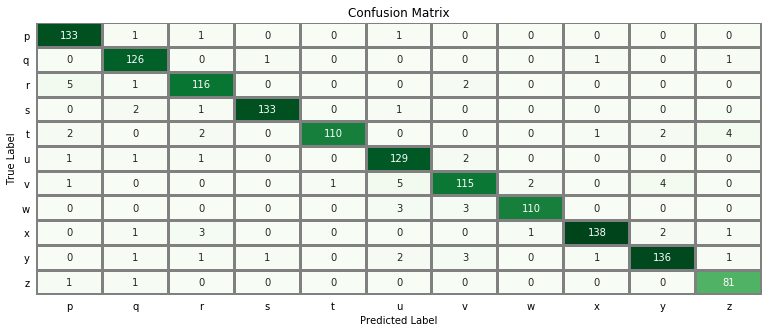
\includegraphics[width=\linewidth]{imgs/model_1.png}
	\caption{Confusion Matrix For the First Model}
	\label{fig:model1}
\end{figure}
This model was the one used for the prediction of the test data.

\section*{Autoencoders}
The autoencoder developed has the objective to reduce the dimension of the data from 784 pixels to 150 pixels and the autoencoder model had 3 hidden layers of 350, 150 and 350 neurons respectively, and all of them were activated using the relu function. In Figure \ref{fig:autoencoder} the difference between the original image and the reconstructionx from the encoded ones can be seen. Visually the difference is minimal to an human eye except from some lost in brightness of the image, to reduction of size is more than 5x, but the quality is more or less mantained, which is a great trade-off, the performance deterioration is checked in the next section.

\begin{figure}[h]
	\centering
	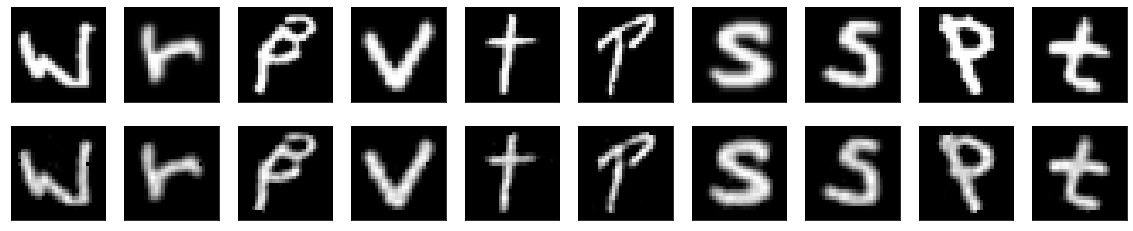
\includegraphics[width=\linewidth]{imgs/autoencoder.png}
	\caption{Original(top) vs Decoded(bottom) images.}
	\label{fig:autoencoder}
\end{figure}

\section*{Classification from encoder}
After the development of the autoencoders the idea was to use the encoded images for the classification task, one could expect the performance to get worse, since some of the information was lost during the encoding. The model was developed taking the encoder part of the autoencoder model and adding 2 Dense Layer of 256 neurons activated with `relu' each. Both layer had a dropout rate of 0.2 to help generalize well. During the training the first two layer (encoder ones) are frozen in order to not influence the encoder's weight. The F$_1$-measure in this case was 0.93, practically we had no loss in performance despite losing information from the encoding. The confusion matrix of the model is in Figure \ref{fig:model2}.
\begin{figure}
	\centering
	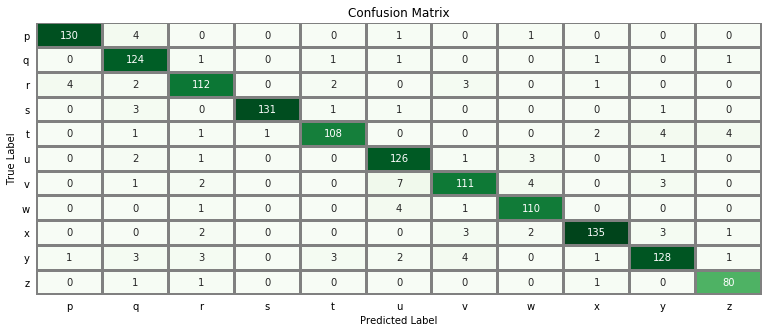
\includegraphics[width=\linewidth,height=4cm]{imgs/model_2.png}
	\caption{Confusion Matrix For the Second Model}
	\label{fig:model2}
\end{figure}

\section*{Conclusion}
The model can be improved by using data augmentation by randomly zooming and tilting the images (a little otherwise a `p' would become a `d'). The encoder worked really well, but the data quantity was really low to improve the model without data augmentation/feature engineering or without using advanced models such as CNNs.\\
There are also some data difficulties such as the third encoded image in the Figure \ref{fig:autoencoder}, it should represent the letter `p', but it is really difficult to tell which letter it actually is. Even a human would have hard time deciding which letter they are (Figure \ref{fig:strange}).

\begin{figure}[!b]
	\centering
	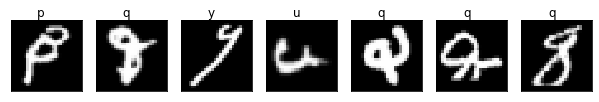
\includegraphics[width=\linewidth, height=1.5cm]{imgs/strange_letters.png}
	\caption{Examples of Confusing Alphabets.}
	\label{fig:strange}
\end{figure}

\end{document}
